\documentclass[border=12pt]{standalone}
\usepackage{tikz}
\usepackage{xcolor}
\definecolor{bgOuter}{RGB}{251,239,221}
\definecolor{bgInner}{RGB}{253,246,234}
\definecolor{shadow}{RGB}{216,185,140}
\definecolor{furMain}{RGB}{217,160,103}
\definecolor{furDark}{RGB}{198,139,82}
\definecolor{furLight}{RGB}{244,221,180}
\definecolor{outline}{RGB}{138,90,50}
\definecolor{eye}{RGB}{74,46,30}
\definecolor{nose}{RGB}{92,58,33}
\definecolor{badge}{RGB}{232,120,90}
\definecolor{badgeEdge}{RGB}{200,90,62}
\definecolor{star}{RGB}{253,246,234}
\definecolor{blush}{RGB}{240,170,150}
\begin{document}
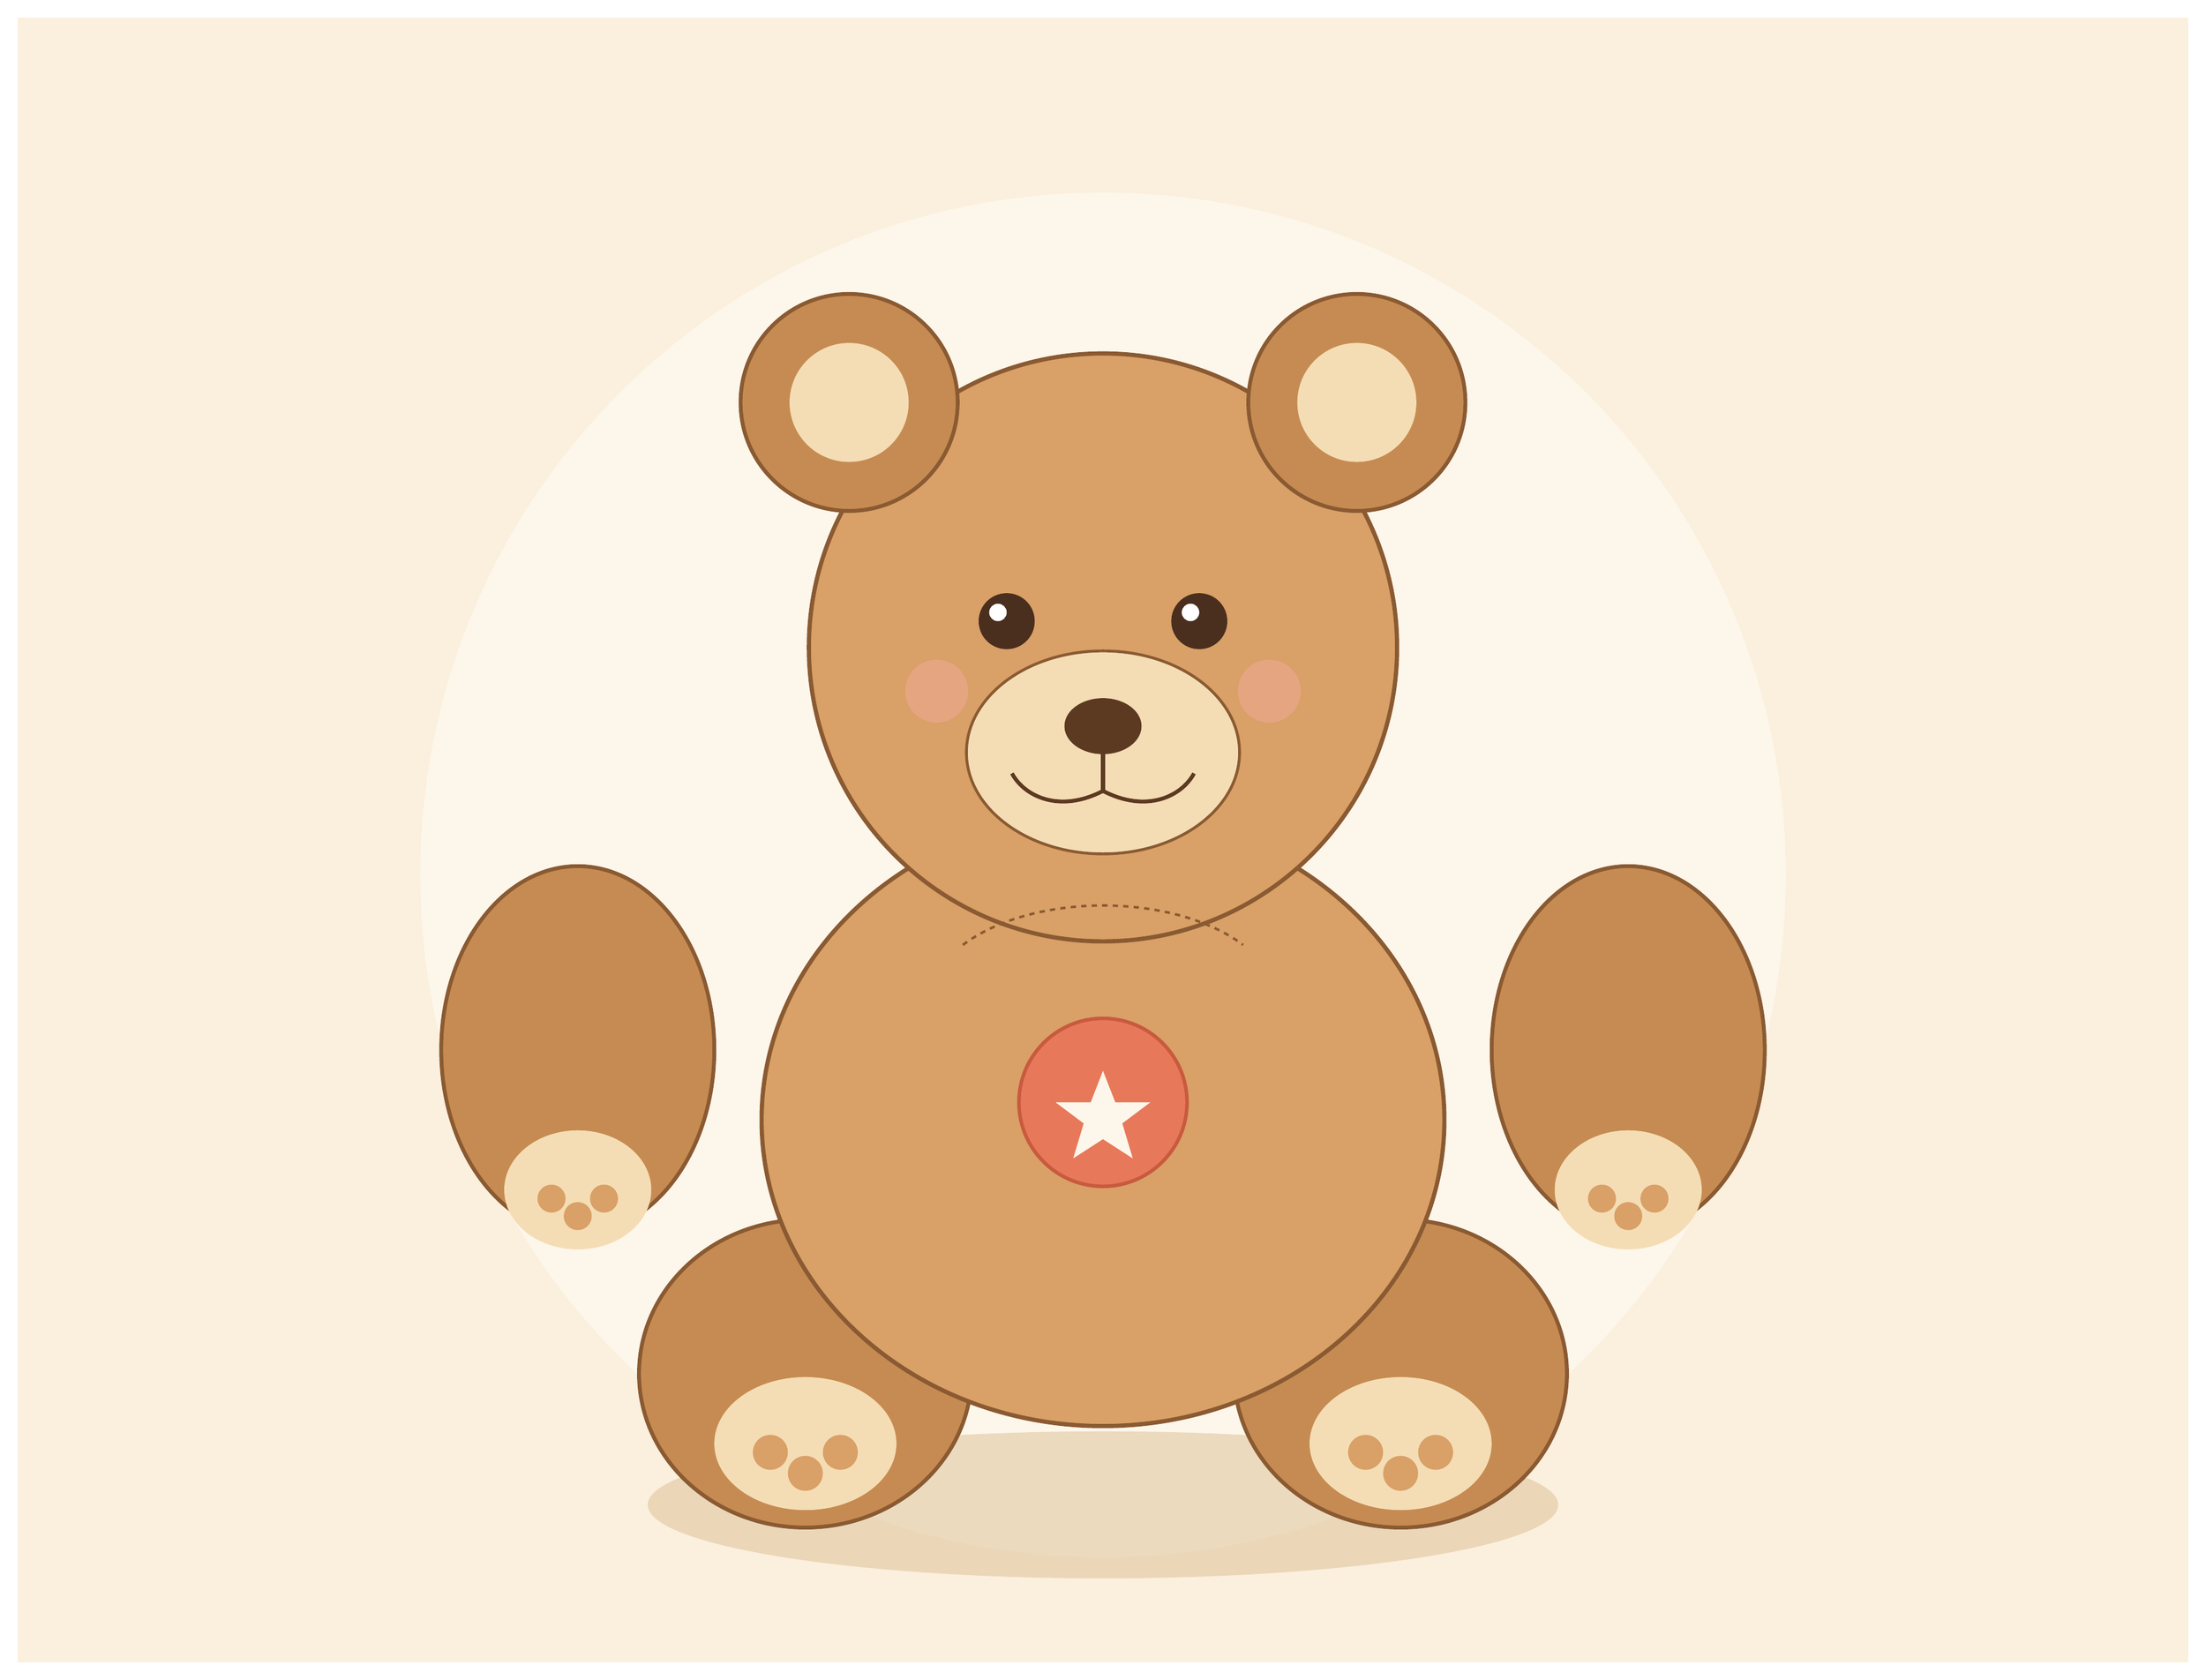
\begin{tikzpicture}[x=1pt,y=1pt]
  \fill[bgOuter] (-20,-20) rectangle (1220,920);
  \fill[bgInner] (600,430) circle (390);
  \fill[shadow,opacity=0.45] (600,70) ellipse (260 and 42);

  % legs
  \fill[furDark] (430,145) ellipse (95 and 88);
  \fill[furDark] (770,145) ellipse (95 and 88);
  \draw[outline,line width=2.2pt] (430,145) ellipse (95 and 88);
  \draw[outline,line width=2.2pt] (770,145) ellipse (95 and 88);
  \fill[furLight] (430,105) ellipse (52 and 38);
  \fill[furLight] (770,105) ellipse (52 and 38);
  \fill[furMain] (410,100) circle (10);
  \fill[furMain] (430,88) circle (10);
  \fill[furMain] (450,100) circle (10);
  \fill[furMain] (750,100) circle (10);
  \fill[furMain] (770,88) circle (10);
  \fill[furMain] (790,100) circle (10);

  % arms
  \fill[furDark] (300,330) ellipse (78 and 105);
  \fill[furDark] (900,330) ellipse (78 and 105);
  \draw[outline,line width=2.2pt] (300,330) ellipse (78 and 105);
  \draw[outline,line width=2.2pt] (900,330) ellipse (78 and 105);
  \fill[furLight] (300,250) ellipse (42 and 34);
  \fill[furLight] (900,250) ellipse (42 and 34);
  \fill[furMain] (285,245) circle (8);
  \fill[furMain] (300,235) circle (8);
  \fill[furMain] (315,245) circle (8);
  \fill[furMain] (885,245) circle (8);
  \fill[furMain] (900,235) circle (8);
  \fill[furMain] (915,245) circle (8);

  % body
  \fill[furMain] (600,290) ellipse (195 and 175);
  \draw[outline,line width=2.4pt] (600,290) ellipse (195 and 175);

  % chest badge
  \fill[badge] (600,300) circle (48);
  \draw[badgeEdge,line width=2pt] (600,300) circle (48);
  \fill[star] (600,318) -- (607,300) -- (627,300) -- (611,288) -- (617,268)
    -- (600,279) -- (583,268) -- (589,288) -- (573,300) -- (593,300) -- cycle;

  % head
  \fill[furMain] (600,560) circle (168);
  \draw[outline,line width=2.4pt] (600,560) circle (168);

  % ears
  \fill[furDark] (455,700) circle (62);
  \fill[furDark] (745,700) circle (62);
  \draw[outline,line width=2.2pt] (455,700) circle (62);
  \draw[outline,line width=2.2pt] (745,700) circle (62);
  \fill[furLight] (455,700) circle (34);
  \fill[furLight] (745,700) circle (34);

  % muzzle
  \fill[furLight] (600,500) ellipse (78 and 58);
  \draw[outline,line width=1.6pt] (600,500) ellipse (78 and 58);

  % eyes
  \fill[eye] (545,575) circle (16);
  \fill[eye] (655,575) circle (16);
  \fill[white] (540,580) circle (5);
  \fill[white] (650,580) circle (5);

  % nose / mouth
  \fill[nose] (600,515) ellipse (22 and 16);
  \draw[nose,line width=2.2pt] (600,500) -- (600,478);
  \draw[nose,line width=2.2pt] (600,478) .. controls (575,465) and (555,475) .. (548,488);
  \draw[nose,line width=2.2pt] (600,478) .. controls (625,465) and (645,475) .. (652,488);

  % cheek blush
  \fill[blush,opacity=0.55] (505,535) circle (18);
  \fill[blush,opacity=0.55] (695,535) circle (18);

  % soft stitch accents
  \draw[outline,line width=1.4pt,dashed]
    (520,390) .. controls (560,420) and (640,420) .. (680,390);
\end{tikzpicture}
\end{document}
